\section{MassSpecGym}
{{\footnotesize
\begin{description}[labelwidth=5em, labelsep=1em, leftmargin=*, align=left, itemsep=0.3em, parsep=0em]
  \item[date:] 2024-12-13
  \item[version:] TODO
  \item[last\_updated:] 2024-12
  \item[expired:] unknown
  \item[valid:] yes
  \item[valid\_date:] TODO
  \item[url:] \href{https://neurips.cc/virtual/2024/poster/97823}{https://neurips.cc/virtual/2024/poster/97823}
  \item[doi:] TODO
  \item[domain:] Cheminformatics; Molecular Discovery
  \item[focus:] Benchmark suite for discovery and identification of molecules via MS/MS
  \item[keywords:]
    - mass spectrometry
    - molecular structure
    - de novo generation
    - retrieval
    - dataset
  \item[summary:] MassSpecGym curates the largest public MS/MS dataset with three standardized tasks-de novo structure generation, molecule retrieval, and spectrum simulation-using challenging generalization splits to propel ML-driven molecule discovery :contentReference[oaicite:3]\{index=3\}.

  \item[licensing:] TODO
  \item[task\_types:]
    - De novo generation
    - Retrieval
    - Simulation
  \item[ai\_capability\_measured:]
    - Molecular identification and generation from spectral data
  \item[metrics:]
    - Structure accuracy
    - Retrieval precision
    - Simulation MSE
  \item[models:]
    - Graph-based generative models
    - Retrieval baselines
  \item[ml\_motif:]
    - Benchmark
  \item[type:] Dataset + Benchmark
  \item[ml\_task:]
    - Generation, retrieval, simulation
  \item[solutions:] TODO
  \item[notes:] Dataset\textasciitilde{}>1M spectra; open-source GitHub repo; widely cited as a go-to benchmark for MS/MS tasks :contentReference[oaicite:4]\{index=4\}.

  \item[contact.name:] Roman Bushuiev
  \item[contact.email:] unknown
  \item[results.links.name:] ChatGPT LLM
  \item[fair.reproducible:] Yes
  \item[fair.benchmark\_ready:] Yes
  \item[ratings.software.rating:] 0
  \item[ratings.software.reason:] Not analyzed.

  \item[ratings.specification.rating:] 9.0
  \item[ratings.specification.reason:] Focused on sound source localization for rodent vocalizations in lab settings; well-scoped.

  \item[ratings.dataset.rating:] 9.5
  \item[ratings.dataset.reason:] 767000 annotated audio segments across diverse conditions. Minor deduction for no train/test/valid split.

  \item[ratings.metrics.rating:] 9.5
  \item[ratings.metrics.reason:] Localization error, precision/recall used

  \item[ratings.reference\_solution.rating:] 7.0
  \item[ratings.reference\_solution.reason:] CNN-based baselines referenced but unclear whether pretrained models or training code are available.

  \item[ratings.documentation.rating:] 2.0
  \item[ratings.documentation.reason:] Poster and paper outline benchmark intent and setup; repo expected but not confirmed in dataset card.

  \item[id:] massspecgym
  \item[Citations:] \cite{neurips2024_c6c31413}
  \item[Ratings:]
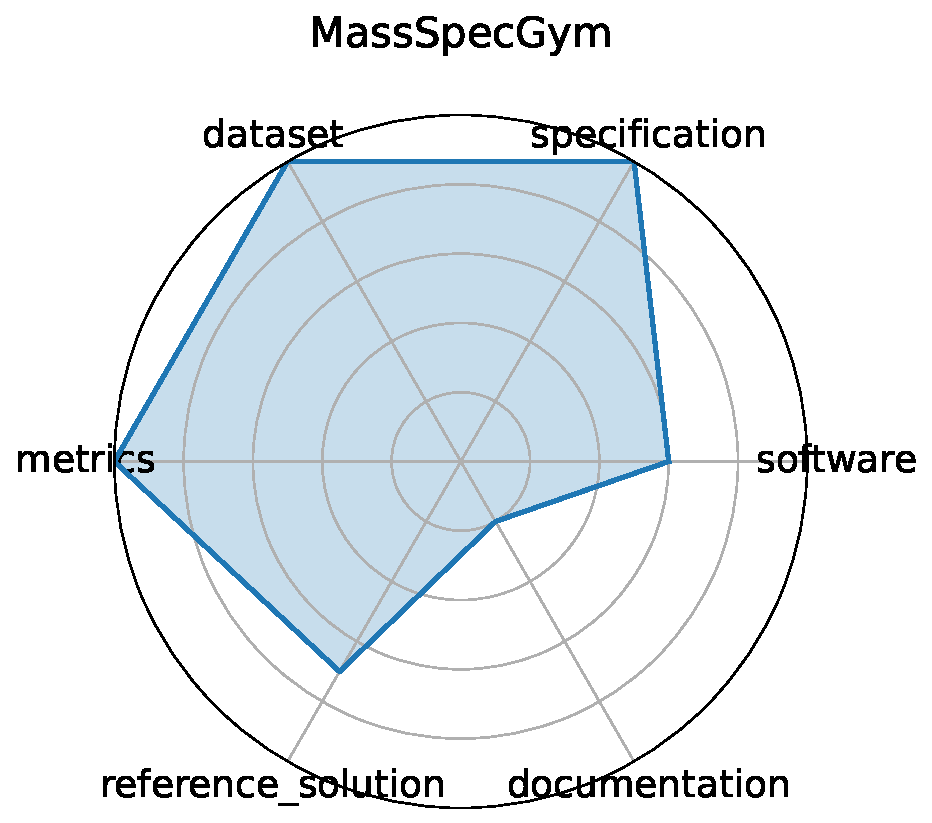
\includegraphics[width=0.2\textwidth]{massspecgym_radar.pdf}
\end{description}
}}
\clearpage